\documentclass[a4paper, 12pt,]{article}


\usepackage{CJKutf8}
\usepackage[colorlinks=true, allcolors=blue]{hyperref}
\usepackage{listings}

\usepackage{tikz}
\usepackage{xcolor}
\usepackage{graphicx}


\definecolor{codegreen}{rgb}{0,0.6,0}
\definecolor{codegray}{rgb}{0.5,0.5,0.5}
\definecolor{codepurple}{rgb}{0.58,0,0.82}
\definecolor{backcolour}{rgb}{0.95,0.95,0.92}

\lstdefinestyle{mystyle}{
    backgroundcolor=\color{backcolour},   
    commentstyle=\color{codegreen},
    keywordstyle=\color{blue},
    numberstyle=\tiny\color{codegray},
    stringstyle=\color{codepurple},
    basicstyle=\ttfamily,
    breakatwhitespace=false,         
    breaklines=true,                 
    captionpos=b,                    
    keepspaces=true,                 
    numbers=left,                    
    numbersep=5pt,                  
    showspaces=false,                
    showstringspaces=false,
    showtabs=false,                  
    tabsize=2
}

\lstset{style=mystyle}
% % this preamble is used for document class: books.
%\usepackage{xeCJK}
\usepackage{graphicx}
\usepackage{float}
%\graphicspath{{./image/}}
\usepackage{graphpap} % 方格紙


\usepackage[most]{tcolorbox}
\usepackage{cleveref}
%\setCJKmainfont{Noto Serif TC}

\tcbset{theostyle/.style={
		enhanced,
		sharp corners,
		attach boxed title to top left={
			xshift=-1mm,
			yshift=-4mm,
			yshifttext=-1mm
		},
		top=1.5ex,
		colback=white,
		colframe=blue!75!black,
		fonttitle=\bfseries,
		boxed title style={
			sharp corners,
			size=small,
			colback=blue!75!black,
			colframe=blue!75!black,
		} 
}}
\tcbset{defstyle/.style={
		enhanced,
		sharp corners,
		attach boxed title to top left={
			xshift=-1mm,
			yshift=-4mm,
			yshifttext=-1mm
		},
		top=1.5ex,
		colback=white,
		colframe=green!50!black,
		fonttitle=\bfseries,
		boxed title style={
			sharp corners,
			size=small,
			colback=green!50!black,
			colframe=green!50!black,
		} 
}}
\tcbset{expstyle/.style={
		enhanced,
		sharp corners,
		attach boxed title to top left={
			xshift=-1mm,
			yshift=-4mm,
			yshifttext=-1mm
		},
		top=1.5ex,
		colback=white,
		colframe=red!70!black,
		fonttitle=\bfseries,
		boxed title style={
			sharp corners,
			size=small,
			colback=red!70!black,
			colframe=red!70!black,
		} 
}}

\newtcbtheorem[number within=chapter]{Thm}{Theorem}{
	theostyle
}{thm}

\newtcbtheorem[number within=chapter]{Def}{Definition}{
	defstyle
}{def}

\newtcbtheorem[number within=chapter]{Exp}{Example}{
	expstyle
}{exp}

\newtcbtheorem[number within = tcb@cnt@Thm]{Lem}{Lemma}{
	theostyle
}{lem}
\newtcbtheorem[number within=tcb@cnt@Thm]{Cor}{Corollary}{
	theostyle
}{cor}

\newtcbtheorem[number within=chapter]{Wng}{Warning}{
	expstyle
}{Wng}

\newtcbtheorem[number within=chapter]{Tip}{Tips}{
	theostyle
}{Tip}
\usepackage[whole]{bxcjkjatype}
\usepackage{ohtex}
\begin{document}
% \begin{CJK*}{UTF8}{}
% \begin{CJK}{UTF8}{gbsn}

% \graphicspath{ {./image/} }
% \setcounter{section}{-1}

\title{Data Structure Homework \#2 \\日本將棋對弈與棋譜瀏覽程式}
\author{Ping-Chen,Chung(鍾秉辰)\\Student ID: 110503007\\Department of Communication Engineering\\National Central University}

	\maketitle
	\tableofcontents
	\newpage
% 	\begin{abstract}
% 	This report introduces the basic structure of neural networks and the C functions of dynamic memory allocation, which is used to precisely manage the memory of the program of neural network XOR operator training program. The program then implements the learnt result to calculate the binary parity checksum of an user-input string. The author then analyzed the graph of the loss function(MSE loss) and proposed the further improvement of this program. 
	    
% 	\end{abstract}
	
	\section{先備知識}
    由於本專案大量的使用日本將棋之日文術語用於命名變數,為求程式之可讀性,在此列出可能會使用到之術語:
	\subsection{棋駒}
	\begin{table}[h]
	    \centering
	    \begin{tabular}{c|c|c|c}
	        棋駒名稱 & 日文簡寫 & 羅馬拼音 & 羅馬簡寫\\
	        \hline
	        步兵 & 步 & fuhyou & fu\\
	        香車 & 香 & kyousha & kyo\\
	        桂馬 & 桂 & keima & kei\\
	        銀將 & 銀 & ginshou & gin\\
	        金將 & 金 & kinshou & kin\\
	        飛車 & 飛 & hishya & hi\\
	        角行 & 角 & kakugyo & kaku\\
	        玉將 & 玉 & gyokushou & gyoku\\
	         \hline
	        と金 & と & tokin & to\\
	        成香 & 杏 & narikyo & narikyo\\
	        成桂 & 圭 & narikei & narikei\\
	        成銀 & 全 & narigin & narigin\\
	        竜王 & 竜 & ryuuou & ryu\\
	        竜馬 & 馬 & ryuuma & uma\\
	    \end{tabular}
	    \caption{棋駒名稱及常用羅馬拼音對照表}
	    \label{tab:my_label}
	\end{table}
	\subsection{術語解釋}
	於此章節,主要介紹於此程式可能會使用到的術語。該術語將會長時間
	\begin{table}[]
	    \centering
	    	\begin{tabular}{c|c|c|l}
	        術語 & 日文 & 羅馬拼音 & 定義\\
	        \hline
	        成變 & なる  & naru  & 友方棋駒到達敵陣三段目時之棋駒升級\\
	        持駒& もちこま & mochikoma& 捕獲的對方持駒列表\\
	        盤面& ばんめん & bannmenn&將棋遊戲盤面\\
	        棋譜 & きふ & kifu& 紀錄對局紀錄之檔案\\
	        手番 & てばん & teban & 現在盤面輪到的對局者\\
	        先手 & せんて & sente&     開局先走棋的對局者(奇數手)\\
	        後手 & ごて & gote& 開局後走棋的對局者(偶數手)\\
	       
	    \end{tabular}
	    \caption{術語名稱及常用羅馬拼音對照表}
	    \label{tab:my_label}
	\end{table}

	

	\subsection{棋譜 / 遊戲紀錄格式}
	In this section, we will introduce how the kifus (or game records ) are stored in Japanese Shogi Association as well as Computer Shogi Association.
	
	\subsubsection{棋譜格式}


    \lstset{escapeinside=``}
    \subsubsection{KIF 記譜格式}
    KIF記譜格式為傳統記譜外最普及的將棋棋譜格式,因篇幅所現不仔細講解,並列格式如下:
    \lstinputlisting[language=C]{kifu/kif.txt}
	\subsubsection{CSA 記譜格式}
	根據計算機將棋協會(コンピュータ将棋協会, Computer Shogi Association)所制定之計算機通用棋譜紀錄格式\cite{CSA},在此列出CSA棋譜之記錄格式:
	
	
	
	\paragraph{盤面} 紀錄當時棋局的盤面。其要點如下所示:
	\begin{itemize}
	
	    \item 各棋駒由下表賦予其英文代號:
	    \begin{table}[h]
	        \centering
	        \begin{tabular}{c|c|c|c|c|c|c|c}
	           步  &香 & 桂 &銀&金&飛&角&玉/王 \\
	           \hline
	             FU  &KY & KE &GI&KI&HI&KA&OU\\
	            \hline
	            と  &杏 & 圭 &全&&竜&馬\\
	            \hline
	            TO &NY & NK &NG& &RY&UM\\
	        \end{tabular}
	        \caption{KIF代號對照表}
	        \label{tab:my_label}
	    \end{table}
	    \item 每個CSA檔案可包含一(可選的)盤面作為初始盤面。若無指定,將會預設為一般的初始盤面。

	    \item 若要記錄持駒,可使用如 \verb|P[先後手]00[棋駒代號]| 之方式。 
	    
	\end{itemize}
	\paragraph{棋譜} 移動的棋譜將以以下物件生成:
	    \begin{itemize}
	        \item 手番: 以\verb|+|或是\verb|-| 表示。
	        \item 初始座標:將棋駒移動前的座標以[筋][段]之方式表示。
	        \item 結束座標:將棋駒結束移動座標以[筋][段]之方式表示。
	    \end{itemize}
	\paragraph{終局} 終局時,可以 \verb|%TORYO| 表記棋局結束。
	以下為標準的CSA 棋譜表示法:
	\lstinputlisting[]{kifu/csa.txt}
	\subsubsection{SFEN 記譜格式\cite{SFEN}}
	\label{chap:sfen}
	SFEN 格式全稱為 \textit{Shogi Forsyth-Edwards Notation} ,係仿製西洋棋之 \textit{Forsyth-Edwards Notation} \cite{FEN} 所定義的盤面標示格式。該類型之棋譜可用於紀錄當前盤面,且無須紀錄該盤面自初手開始的棋局變化。所需之欄位如下所示:
	\paragraph{盤面}
	紀錄當時棋局的盤面。其要點如下所示:
	\begin{itemize}
	    \item 棋譜輸入自左到右,由上到下;對應於傳統將棋座標中,自9一開始到1九結束。
	    \item 各棋駒由下表賦予其英文代號:
	    \begin{table}[h]
	        \centering
	        \begin{tabular}{c|c|c|c|c|c|c|c}
	           步  &香 & 桂 &銀&金&飛&角&玉/王 \\
	           \hline
	             P  &L & N &S&G&R&B&K
	        \end{tabular}
	        \caption{SFEN代號對照表}
	        \label{tab:my_label}
	    \end{table}
	    \item 若該棋駒為昇變棋駒,則於該代號前加上一個 \verb|+| 號標記。
	    \item 無棋駒的連續 $n$ 個空格以數字$n$表示。
	    \item 一行以九個棋駒為限,行與行間用 \verb|/| 區隔。若令一行中有 $m$ 個英文字元與 $n$ 個數字,分別為$n_1, n_2 \cdots$,則每一行有以下限制:
	    $$
	    m + \sum n_i = 9
	    $$
	\end{itemize}
	\paragraph{手番}記錄該盤面下一手的所屬。
	\paragraph{持駒}記錄先後手的持駒。大寫的代號為先手持駒,小寫則為後手持駒。所有的持駒將會以無空白字串儲存。若一方持有 $n$ 個相同持駒,則在對應的代號上加上數字 $n$ 。
	\paragraph{手數}紀錄當時的手數(自棋局開始後經過的棋步數量)。
	
    \subsection{初手局面}
    此為將棋棋局的最初局面,如下圖:
    \begin{figure}[h]
        \centering
          \shogiban{\hirate}
        \caption{棋局初手局面}
        \label{fig:my_label}
    \end{figure}
    該盤面可使用SFEN記譜表示為
    \begin{lstlisting}
lnsgkgsnl/1r5b1/ppppppppp/9/9/9/PPPPPPPPP/1B5R1/LNSGKGSNL b - 1
\end{lstlisting}\newpage
	
% 	\section{Theoretical Background of Neural Network}
    In this section, we're going to introduce the definition of neural networks, and its implementations in C as a library.
	\subsection{Shogi}
	\subsection{Term Explanation}
	\subsection{}
    

	\newpage
		\section{程式}
	於此章節,我們在此簡要敘述本程式使用到的函式及預定義的常數。
	\subsection{實作功能}
	\begin{itemize}
	    \item 棋駒移動
	    \item 棋駒昇變
	    \item 駒台與持駒打入
	    \item 棋譜輸出
	    \item 輸出一般網站可使用之棋譜(sfen)
	\end{itemize}
	\subsection{預定義常數}
	\lstinputlisting[language=C]{src/const.c}
	\subsection{結構}
	於此章節,我們定義此程式使用的結構體如下:
\lstinputlisting[language=C]{src/structures.c}	
	\subsection{函式}
\lstinputlisting[language=C]{src/functions.c}
	

	\subsection{編譯方式}
	    請下載並開啟本專案資料夾,並輸入以下指令:
	    \begin{lstlisting}[language=sh,caption=Compile Parameters]
$ make  
$ ./main	     \end{lstlisting}

\subsection{棋譜輸出格式}
於本專案中,遊戲過程將於退出時紀錄於\verb|./sfenlist|。該格式之讀法請參照\autoref{chap:sfen},以一行為單位為一手的盤面。範例輸出如下:
\begin{lstlisting}
lnsgkgsnl/1r5b1/ppppppppp/9/9/9/PPPPPPPPP/1B5R1/LNSGKGSNL b - 1
lnsgkgsnl/1r5b1/ppppppppp/9/9/2P6/PP1PPPPPP/1B5R1/LNSGKGSNL w - 2
lnsgkgsnl/1r5b1/pppppp1pp/6p2/9/2P6/PP1PPPPPP/1B5R1/LNSGKGSNL b - 3
lnsgkgsnl/1r5+B1/pppppp1pp/6p2/9/2P6/PP1PPPPPP/7R1/LNSGKGSNL w B 4
lnsgkg1nl/1r5s1/pppppp1pp/6p2/9/2P6/PP1PPPPPP/7R1/LNSGKGSNL b Bb 5
lnsgkg1nl/1r5s1/pppppp1pp/6p2/4B4/2P6/PP1PPPPPP/7R1/LNSGKGSNL w b 6
\end{lstlisting}

\subsection{程式使用方式}



\subsubsection{開始新局面}
請執行以下指令
\begin{lstlisting}[language=sh,caption=Compile Parameters]
$ ./main	     
\end{lstlisting}
以開啟新局面。
進入後,系統將會提示輸入先手方之棋步,請依照以下規則輸入:[初始座標][結束座標][棋駒羅馬簡寫],座標之(1,1)位於棋盤先手方之左上角。\\
範例如下:
\begin{lstlisting}[,caption=Examples of Inputs]
77 76 fu
33 34 fu
88 22 kaku
31 22 gin 
00 55 kaku //`持駒打入,初始座標為00`
\end{lstlisting}
若棋駒可昇變,將會提示
\begin{lstlisting}[]
`<<成りますか?>>(naru, narazu)`
\end{lstlisting}
請輸入\verb|naru|以昇變或\verb|narazu|以保持為原棋駒。\\
若要悔棋,可以輸入
\begin{lstlisting}[]
revert
\end{lstlisting}
;若要退出,請輸入
\begin{lstlisting}[]
quit
\end{lstlisting}
。退出之後,此程式會紀錄該次棋局之棋譜,存放於
\begin{lstlisting}[]
./kifu.sfenlist
\end{lstlisting}
存放,待回放使用。
\subsubsection{單行sfen棋譜讀入}
請執行以下指令
\begin{lstlisting}[language=sh,caption=Compile Parameters]
$ ./main --readsfen ${SFENFILE_LOCATION}	     
\end{lstlisting}
以使用sfen格式繼續中斷的棋局,並繼續遊玩。
您可以使用 \\https://lishogi.org/analysis/ 以生成一個新盤面。
\subsubsection{棋譜瀏覽}
本棋譜瀏覽功能僅限讀入本程式之 \verb|sfenlist| 檔案。請使用
\begin{lstlisting}[language=sh]
$ ./main --replay ${SFENLIST_FILE_LOCATION}	     
\end{lstlisting}
並使用 \verb|f, b| 前後瀏覽。退出時按下 \verb|q| 即可。 \newpage
% 		\section{實作問題與未來展望}
	由於有限的時間,仍有部份功能尚未實作,詳列如下:
	\begin{itemize}
	    \item 傳統棋譜表示\\
	    由於棋譜
	\end{itemize}\newpage
% 	\section{Analysis}
		\subsection{Loss Function}
	From the reference \cite{ref3}, we can know that there exist various ways to evaluate the accuracy of a neural network. For simplicity, this program uses MSE (Mean-Square-Error) to be our loss function to evaluate the accuracy of the neural network. The equation is shown below:
	\begin{equation}
	    \textrm{MSE} = (\frac{1}{n})\sum_{i=1}^{n}\left(y_i - \hat{y_i}\right)^2  
	\end{equation}
	where $y_i$ is the actual training output and $\hat{y_i}$ is the desired output.   
	\subsection{Graph Display}
	The graph below shows the loss function with sample training iterations (30000 times). 
	\begin{figure}[h]
	    \centering
	    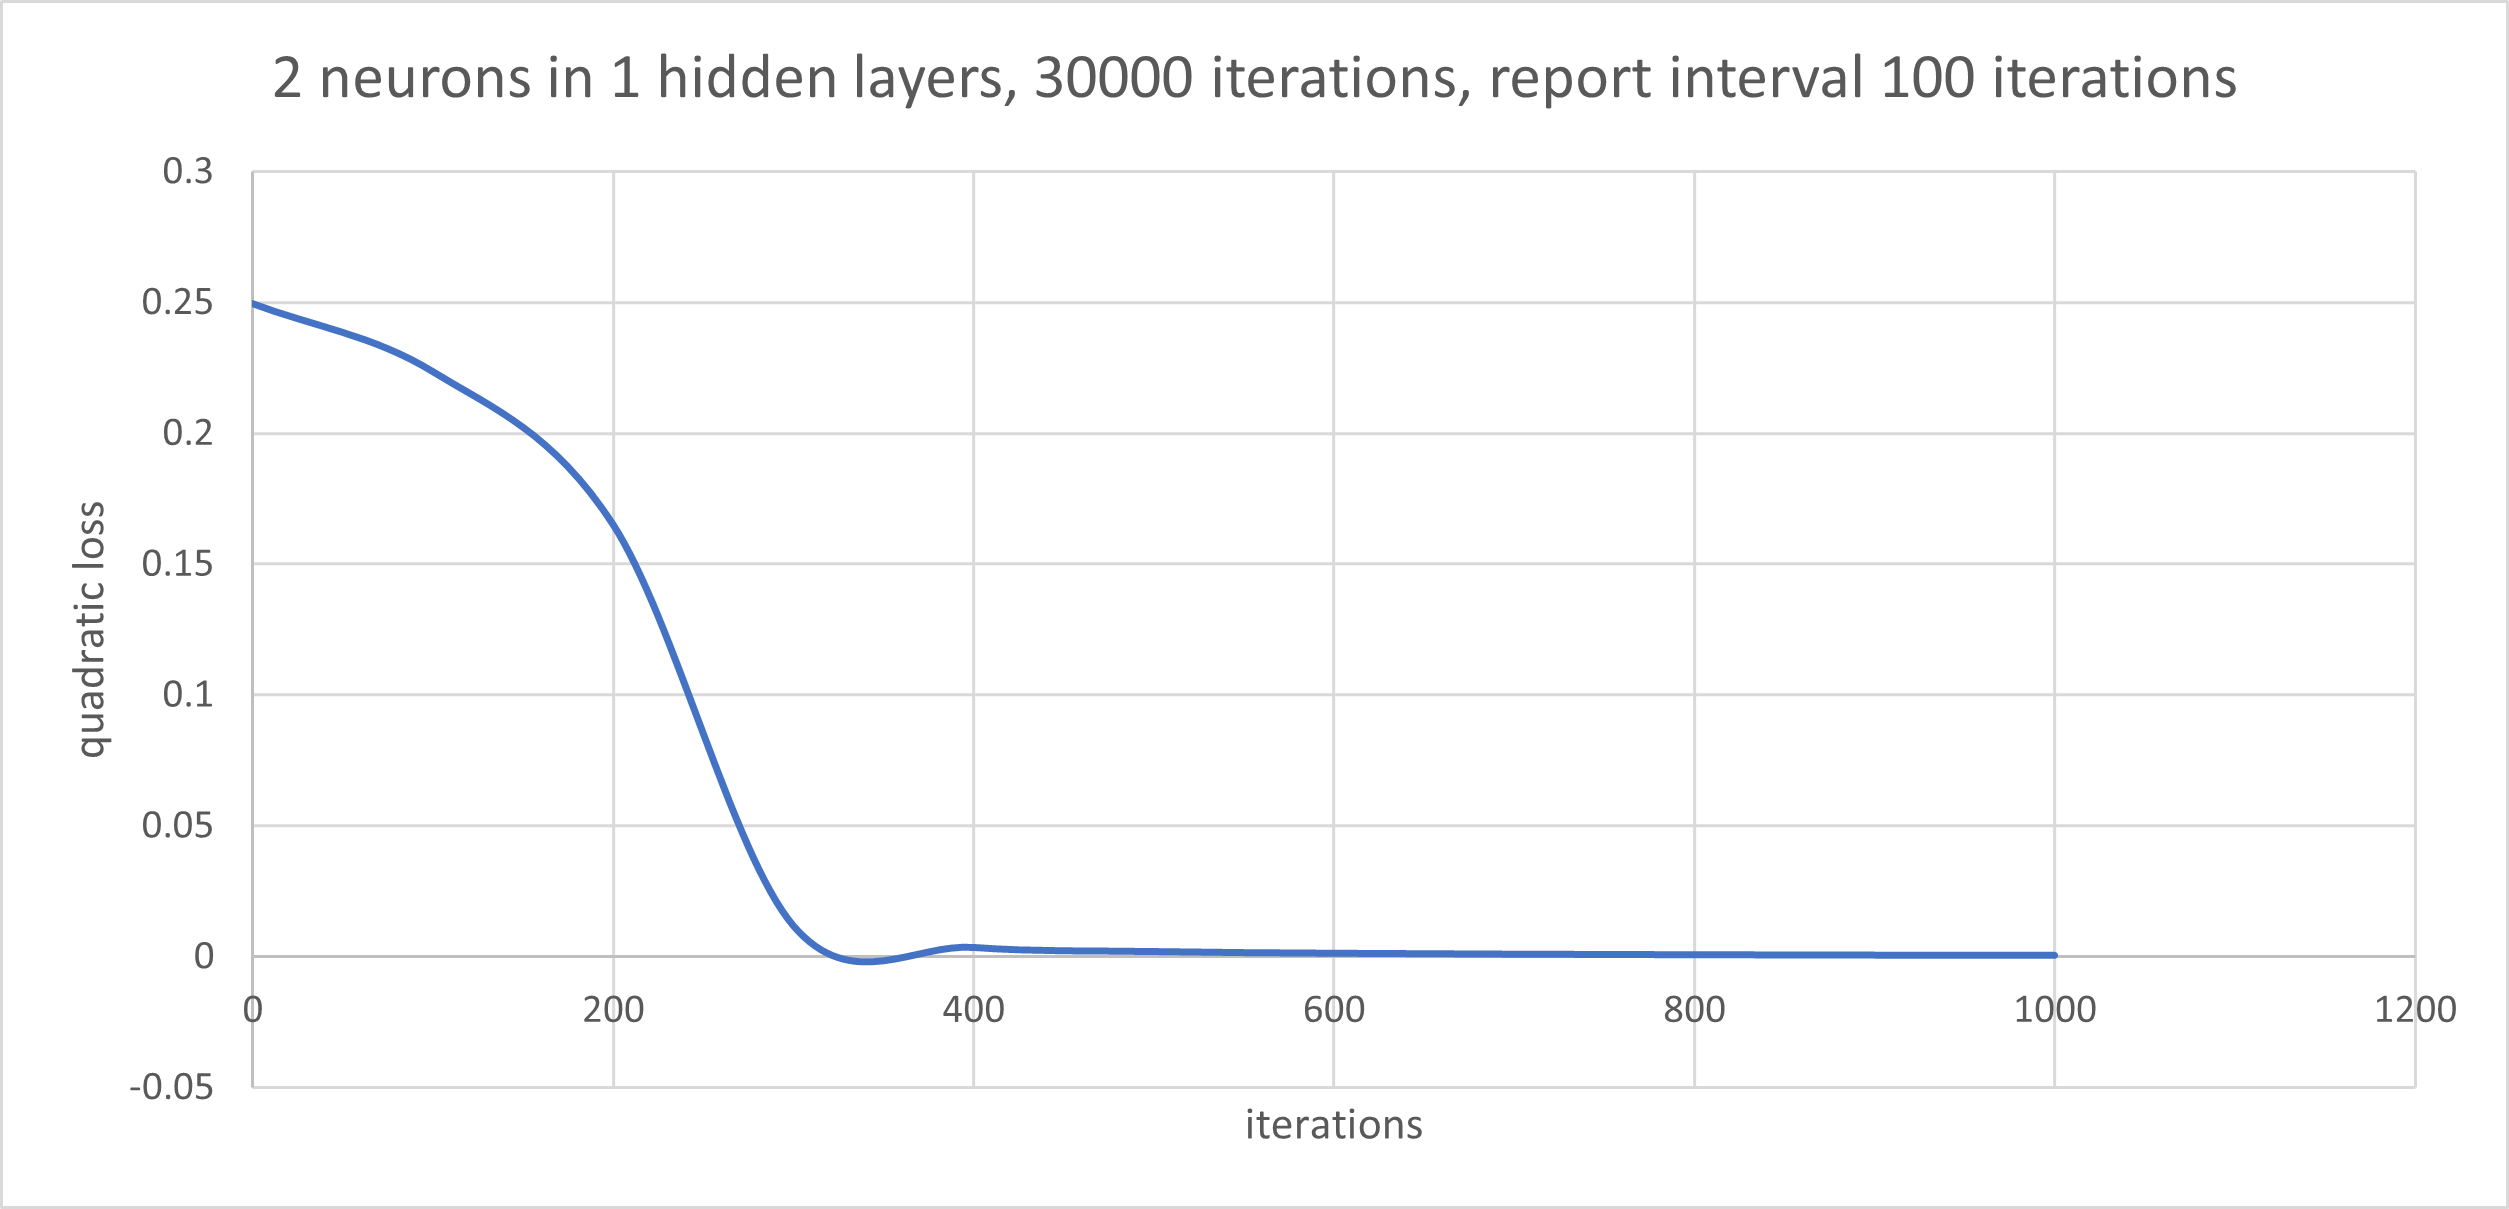
\includegraphics[width=1\textwidth]{image/2in1.png}
	    \caption{Graphs of Loss Function: MSE v.s. iterations}
	    \label{fig:my_label}
	\end{figure}
	\\Note that this graph only shows up to 1000 iterations since the value after 1000 iterations approaches zero and is trivial. The graph at first reached its highest value (approximately 0.25), and then gradually falls down to zero with the increase of training epochs. 
	\subsection{Further Improvement}
	Although the program has been successfully executed, there are still some issues to be fixed, listed below:
	\begin{itemize}
	    \item a CSV output of the loss function could be added when training completes.
	    \item Data storage of bits can be reduced to \lstinline{bool} array instead of \lstinline{char} array to reduce memory. 
	    \item In \lstinline{void getBitString()} : the string of bits can be the function's return value. Doing this may clarify the workflow of  \lstinline{void getRealAns()} and \lstinline{void getTrainAns()}. 
	\end{itemize}



	
	
	
    % \bibliographystyle{alpha}
% 	\bibliography{ref}




	\begin{thebibliography}{99}  
	
	\bibitem{CSA} http://www2.computer-shogi.org/protocol/record\_v22.html
	\bibitem{FEN} https://en.wikipedia.org/wiki/Forsyth\%E2\%80\%93Edwards\_Notation
	\bibitem{SFEN} https://en.wikipedia.org/wiki/Shogi\_notation#SFEN
	
	
	
		
	\end{thebibliography} 


% \end{CJK}

\end{document}